% vim: expandtab softtabstop=2 shiftwidth=2 foldmethod=marker spell

\section{Troubleshooting the songbot}

\subsection{Normal users cant add songs}

Step one, use the command \lstinline{!sl}, which should return the link to the songlist. If it does, check to see if the queue is on.
\begin{figure}[ht!]
  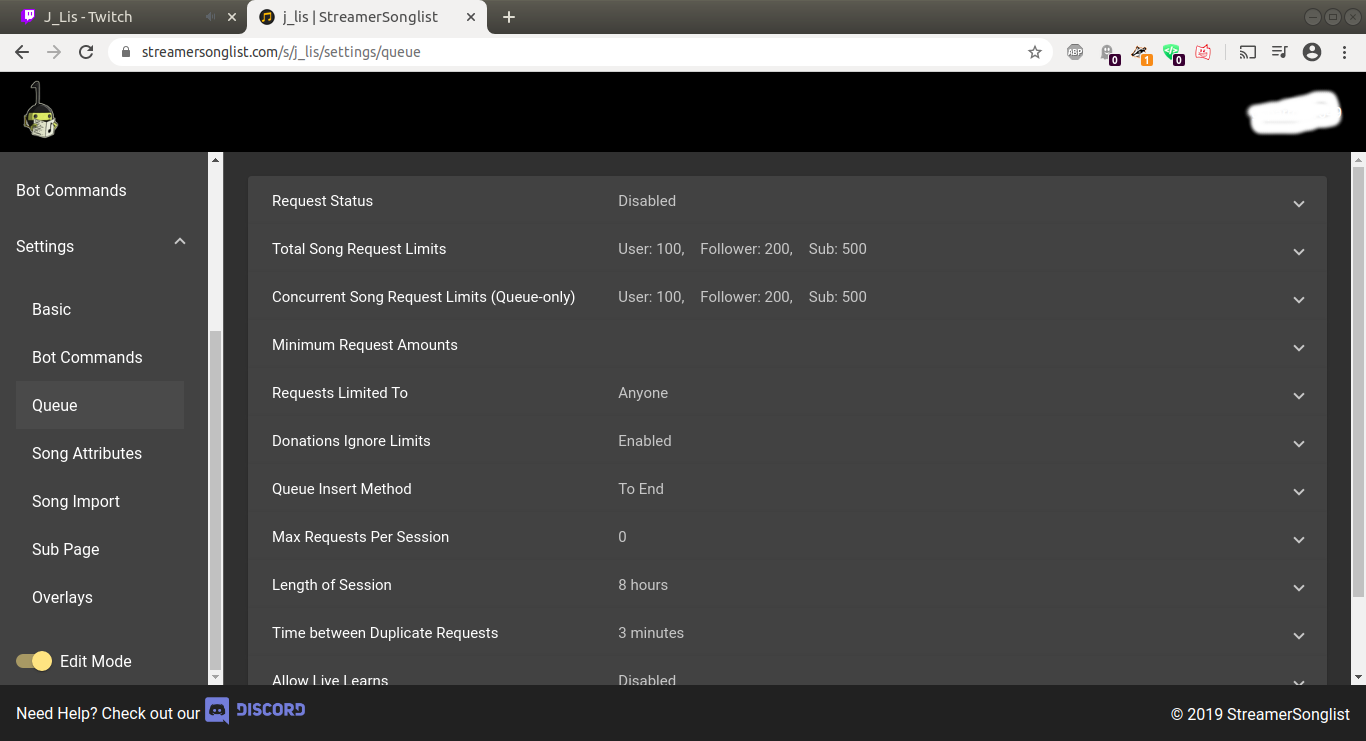
\includegraphics[width=\linewidth]{src/troubleshooting_songbot/bot_off.png}
  \caption{The webpage with the songbot turned off}
  \label{bot is off}
\end{figure}

When the command \lstinline{!sl} does not work, check to see if the bot is connected to chat.
\begin{figure}[ht!]
  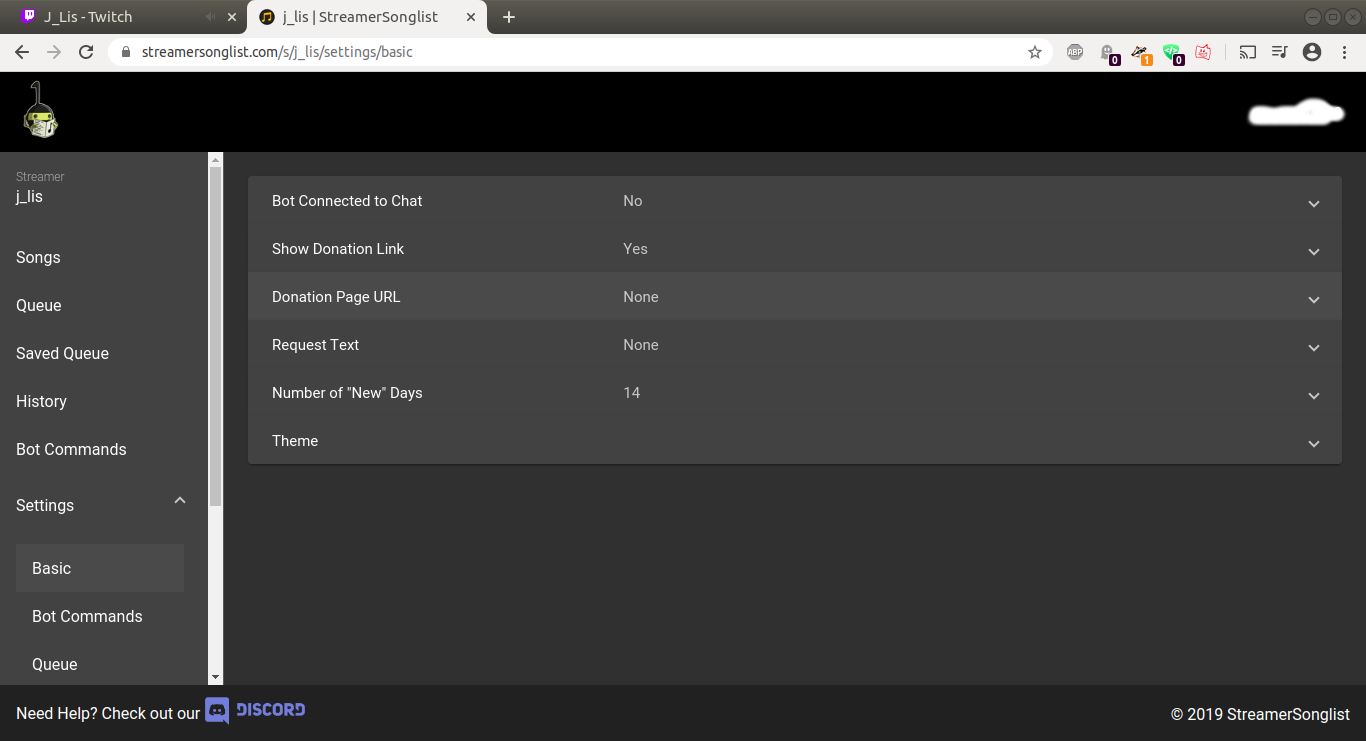
\includegraphics[width=\linewidth]{src/troubleshooting_songbot/bot_disconnected.png}
  \caption{The webpage with the songbot disconnected}
  \label{bot disconnected}
\end{figure}
When the bot is connected and it did not work, check the command list. songlist and songrequest have been known to get turned off by mods unknown.
\begin{figure}[ht!]
  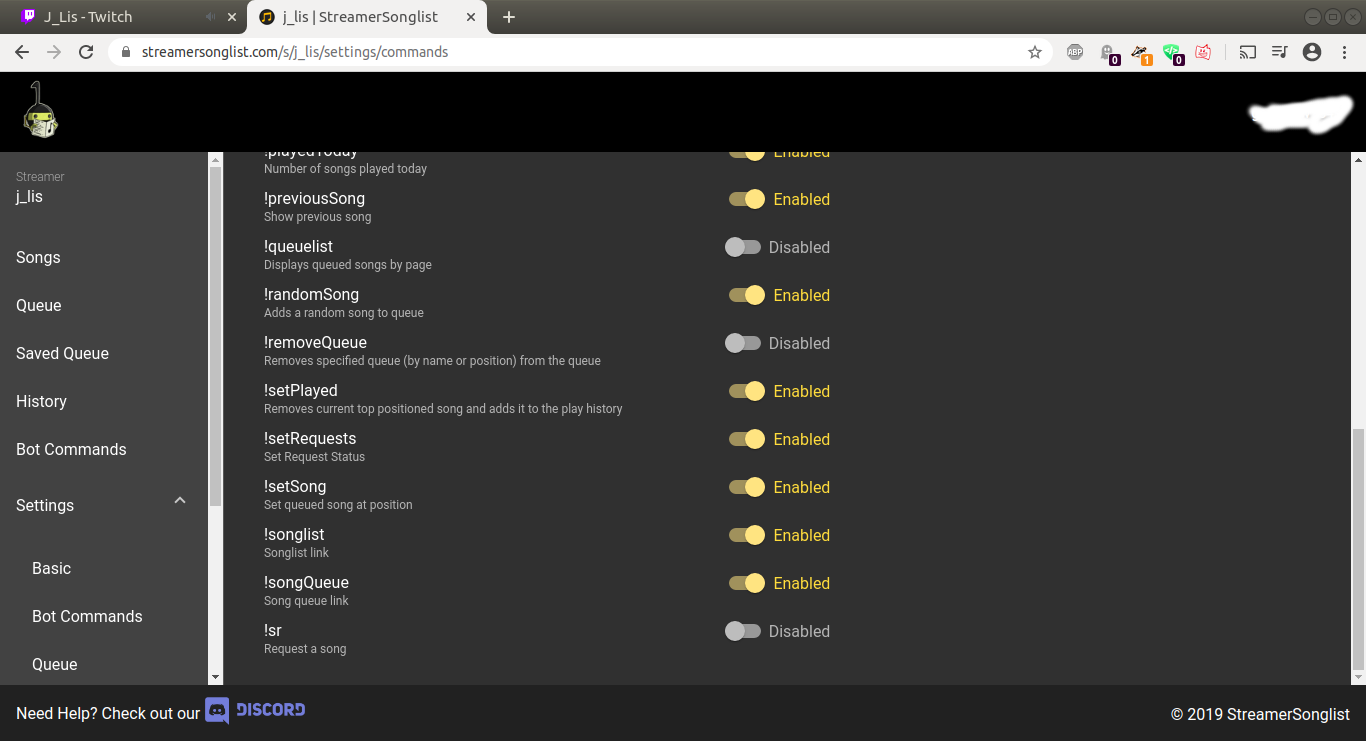
\includegraphics[width=\linewidth]{src/troubleshooting_songbot/songlist_commands_off.png}
  \caption{The webpage with the commands turned off}
  \label{commands off}
\end{figure}

\newpage
\subsection{What it is supposed to look like}
\begin{figure}[ht!]
  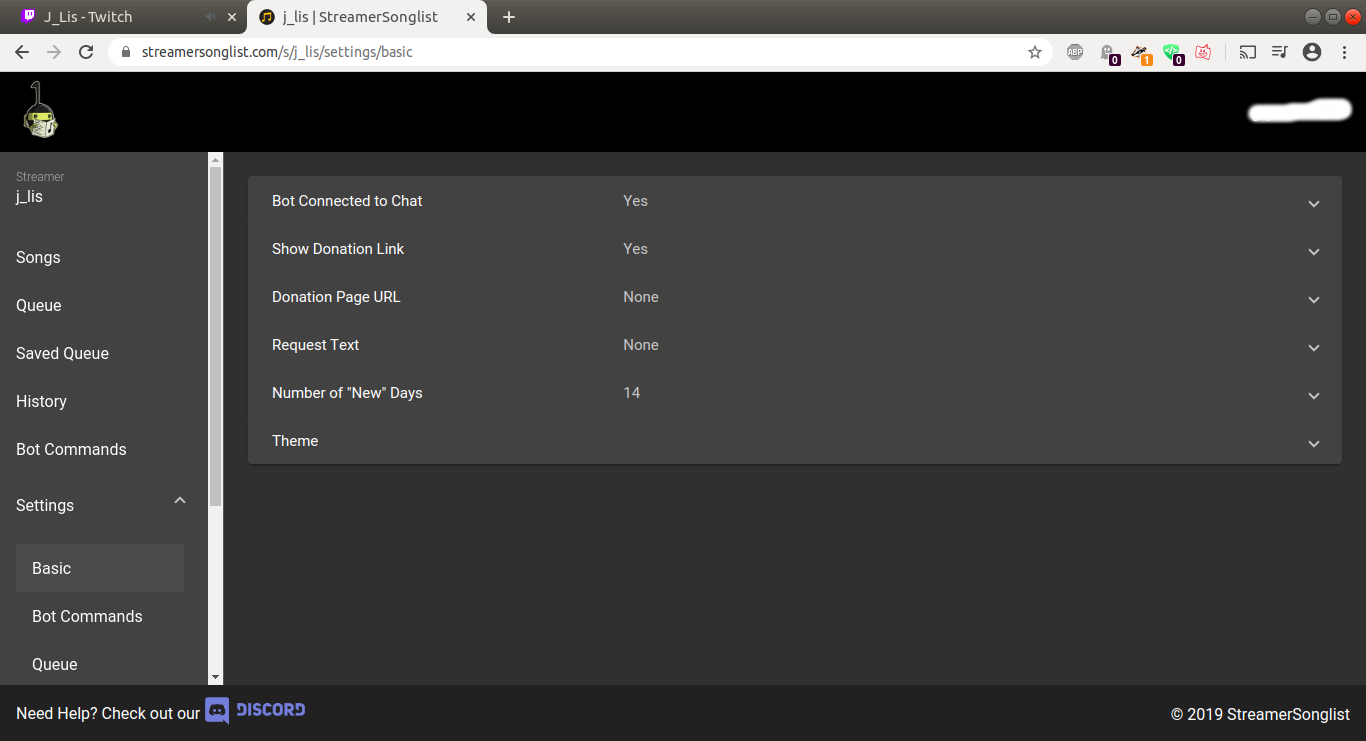
\includegraphics[width=\linewidth]{src/troubleshooting_songbot/bot_connected.png}
  \caption{The webpage with the songbot connected}
  \label{bot disconnected}
\end{figure}
\begin{figure}[ht!]
  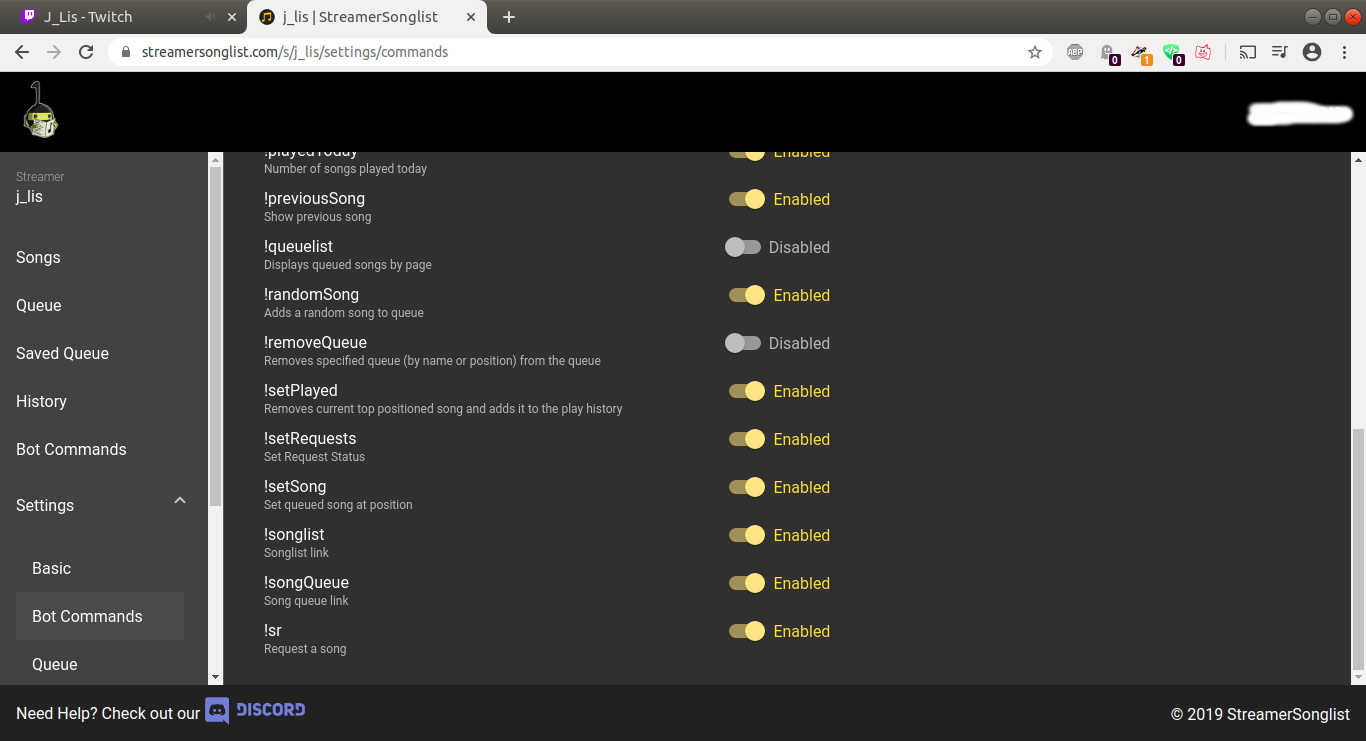
\includegraphics[width=\linewidth]{src/troubleshooting_songbot/songlist_commands_on.png}
  \caption{The webpage with the commands turned on}
  \label{commands off}
\end{figure}
\begin{figure}[ht!]
  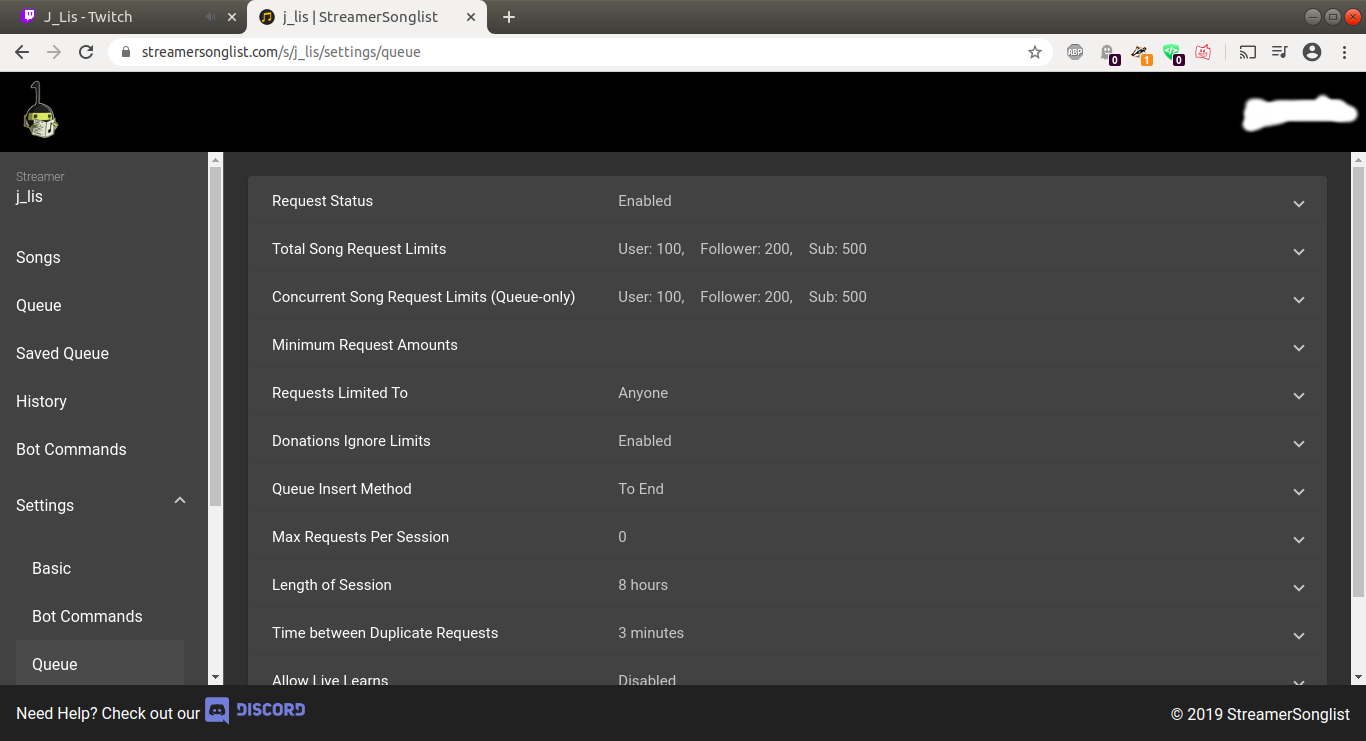
\includegraphics[width=\linewidth]{src/troubleshooting_songbot/bot_on.png}
  \caption{The webpage with the songbot turned on}
  \label{bot is on}
\end{figure}

